\chapter{Aplikace SZDC}
\label{kap6:szdc_app}
Abychom předvedli využití knihovny GTTG, chtěli jsme vybrat existující implementaci nákresných jízdních řádů, na které bychom ukázali, že je naše knihovna dostatečně konfigurovatelná tak, aby umožnila vytvoření nákresného jízdního řádu podle skutečných a~přesně definovaných požadavků. Proto jsme se rozhodli vytvořit aplikaci pro práci s~nakresnými jízdními řády~(cíl \ref{uvod:cil:aplikace}), které jsou vydávány Správou železniční a~dopravní cesty (SŽDC) a~jsou veřejně přístupné~\cite{GVD_njr} spolu s~dalšími pomůckami grafikonu vlakové dopravy nebo se nachází k~nahlédnutí v~příloze práce v~\texttt{/szdc/njr/pdf}. Popíšeme si cestu, jak jsme získali data, která budou při zobrazení v~aplikaci (obrázek \ref{fig:kap6:aplikace_vysledek}) co nejvěrněji odpovídat vzoru zmíněných nákresných jízdních řádů (obrázek \ref{fig:kap6:vzor_gvd}). Nejdříve si ale popíšeme architekturu aplikace a~dva způsoby zobrazení, které aplikace nabízí.

\begin{figure}[!hbt]
	\centering
	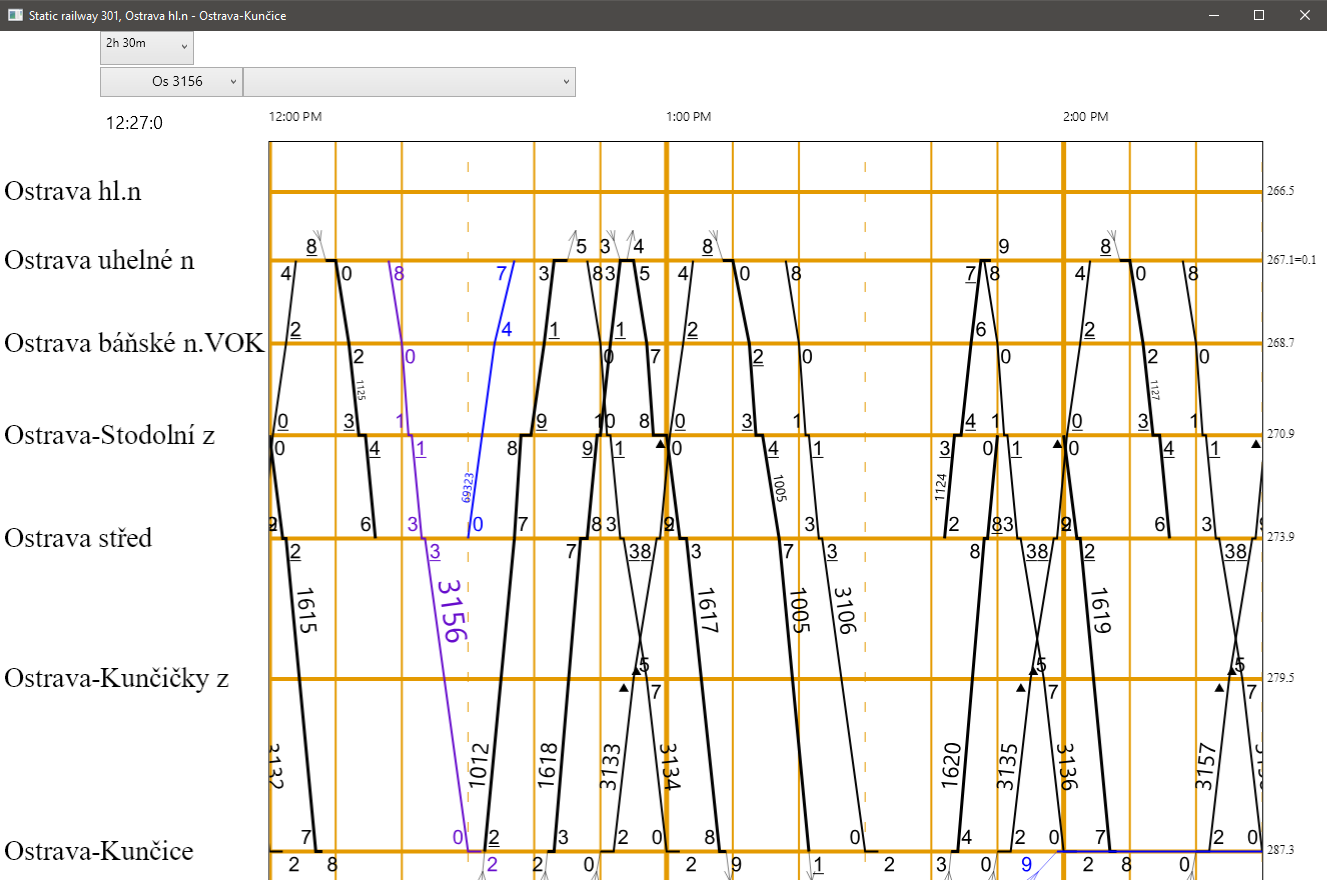
\includegraphics[width=\textwidth]{../img/kap6_szdc_application}
	\caption{Zobrazení nákresného jízdního řádu v~aplikaci}
	\label{fig:kap6:aplikace_vysledek}
\end{figure}

\begin{figure}[!hbt]
	\centering
	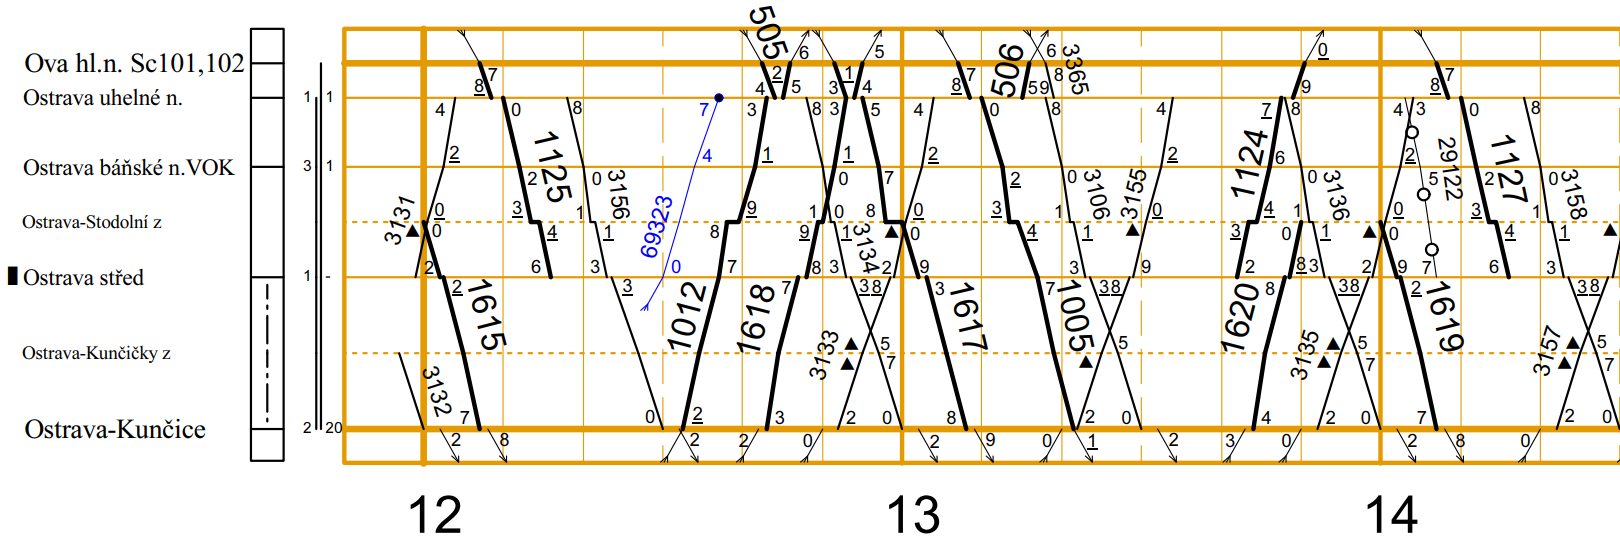
\includegraphics[width=\textwidth]{../img/kap6_njr_vzor}
	\caption{Nákresný jízdní řád vydávaný SŽDC}
	\label{fig:kap6:vzor_gvd}
\end{figure}

\section{Architektura aplikace SZDC}
\label{kap6:szdc_gui_framework}
Aplikaci jsme navrhli tak, aby byla znovupoužitelná v~rámci více GUI frameworků platformy .NET (cíl~\textbf{\color{goalcolor}G2}\ref{uvod:cil:aplikace:vice_gui}). Možnost tohoto návrhu jsme si ověřili na existující a~dostatečně složité aplikaci Core2D~\cite{Core2D}, která tento požadavek splňuje. Aplikaci SZDC jsme rozdělili na projekty, uvedené na obrázku \ref{fig:kap6:szdc_structure}, podobným způsobem jako ve zmíněné aplikaci. V~rámci co největší přenositelnosti jsou projekty aplikační logiky a~jejího modelu (\texttt{SZDC.Editor} a~\texttt{SZDC.Model}) implementovány vůči rozhraní .NET Standard. Model aplikace je rozšířením modelu z~\texttt{GTTG.Model}. Jako zdroj dat používá aplikace připojení k~databázi, které je spravováno v~projektu \texttt{SZDC.Data}, je ale možné pracovat s~daty i~z~jiných zdrojů. V~rámci práce s~daty existují pomocné nástroje jako \texttt{SZDC.JsonParser}. Jako GUI framework aplikace jsme zvolili WPF, určené pro běhové prostředí .NET Framework 4.7.2. Vedle WPF by bylo možné aplikaci použít i~v~GUI frameworku Avalonia~\cite{Avalonia} nebo Xamarin.Forms. V~následujících podkapitolách si všechny tyto projekty více popíšeme.

\begin{figure}[!hbt]
	\centering
	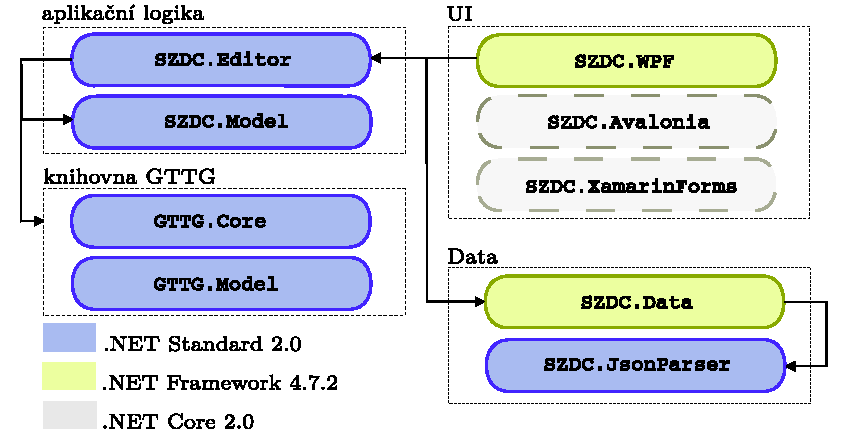
\includegraphics[width=\textwidth]{../img/kap6_szdc_structure}
	\caption{Rozdělení aplikace SZDC do projektů}
	\label{fig:kap6:szdc_structure}
\end{figure}

\subsection*{SZDC.Editor}
Aplikace umožní uživateli zobrazit více oken s~nákresnými jízdními řády zároveň, každé umožňující práci s~nákresným jízdním řádem v~jednom ze dvou módů, které jsme podle \ref{uvod:cil:aplikace} chtěli vytvořit:

\begin{enumerate}
\item Mód k~prohlížení nákresných jízdních řádů SŽDC, který nazveme jako \textit{statický} (cíl~\textbf{\color{goalcolor}G2}\ref{uvod:cil:aplikace:staticke_zobrazeni})
\item Mód simulující provoz na trati, který označíme jako \textit{dynamický} -- komponenta s~nákresným jízdním řádem se periodicky obnovuje, aby odpovídala současnému časovému intervalu několika hodin. Uživatel může modifikovat průběh jízdy vlaku a~tyto změny jsou viditelné mezi více okny v~tomto módu (cíl~\textbf{\color{goalcolor}G2}\ref{uvod:cil:aplikace:dynamicke_zobrazeni}).
\end{enumerate}
\newpage
Z~pohledu uživatele si tyto módy více popíšeme v~uživatelské dokumentaci \ref{kap6:szdc:user_doc}. Pro rozdělení aplikační logiky, nacházející se na obrázku \ref{fig:kap6:szdc_application_logic}, je existence těchto dvou módů důležitá -- každý zobrazuje podobný obsah, ale nabízí různou úroveň jeho modifikace.

\begin{figure}[!hbt]
	\centering
	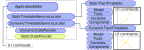
\includegraphics[width=\textwidth]{../img/kap6_szdc_application_logic}
	\caption{Rozdělení aplikační logiky}
	\label{fig:kap6:szdc_application_logic}
\end{figure}

Základem aplikační logiky je třída \texttt{ApplicationEditor}. Pokud například \linebreak z~uživatelského rozhraní klikneme na tlačítko k~otevření nákresného jízdního řádu ve statickém módu, \texttt{ApplicationEditor} vytvoří, nastaví a~vrátí instanci \linebreak \texttt{StaticTrainTimetable}, která je základní třídou nákresného jízdního řádu ve statickém módu. Třída \texttt{StaticTrainTimetable} obsahuje tyto části:

\begin{enumerate}
	\item	Nástroje knihovny GTTG jako \texttt{GraphicalComponent} nebo \newline\texttt{DrawingManager}
	\item 	Model a~view model nákresného jízdního řádu rozšiřující \texttt{GTTG.Model}
	\item	Implementace factory rozhraní view modelů z~\ref{kap4:view_model_factory_impl} v~\texttt{FactoriesCollector}
	\item	Nástroje ve třídě \texttt{ToolsCollector} určené pro práci s~nákresným jízdním řádem, obsahující například:
			\begin{enumerate}
				\item \texttt{CurrentDateTimeTool} převádějící pozici kurzoru myši na časový údaj
				\item \texttt{TrainViewSelectionTool} zajišťující výběr zvýrazňovaného vlaku vyneseného do popředí
				\item \texttt{ViewTimeModifierTool} umožňující nastavení časových intervalů komponenty
			\end{enumerate}
	\item	Komponenty uživatelského rozhraní ve třídě \texttt{ComponentsCollector}:
			\begin{enumerate}
				\item \texttt{TrainTimetableComponent} představuje komponentu nákresného \linebreak jízdního řádu
				\item \texttt{TimeSidebarComponent} představuje horizontální osu časových údajů nad nákresným jízdním řádem
				\item \texttt{RailwayDistanceSidebarComponent} je sloupec kilometrických poloh dopravních bodů na trati
				\item \texttt{StationNamesComponent} představuje sloupec názvů dopravních bodů
			\end{enumerate}
\end{enumerate}

Inicializace \texttt{StaticTrainTimetable} a~jeho částí probíhá přes \textit{dependency injection} framework \textit{Autofac}~\cite{Autofac}. Nemusíme tak složitě inicializovat třídy používané v~\texttt{StaticTrainTimetable} sekvencí konstruktorů, ale inicializace proběhne mimo náš kód. Ukažme si, jak inicializace probíhá. \texttt{StaticTrainTimetable} přímo využívá \texttt{GraphicalComponent} k~modifikacím a~existuje mnoho dalších částí třídy, například \texttt{HitTestManager} nebo \texttt{CurrentTimeTool}, které chtějí získat instanci \texttt{GraphicalComponent} jako implementované rozhraní \texttt{IViewProvider}. \newline \texttt{ApplicationEditor} obsahuje \texttt{StaticTimetableServiceLocator}, spravující registraci nástrojů, které se v~\texttt{StaticTrainTimetable} inicializují. Přidáme do něj \texttt{GraphicalComponent}:

\begin{csharpcode}
public class CoreModule : Module {

  protected override void Load(ContainerBuilder builder) {

   builder
	.RegisterType<GraphicalComponent>()
	.AsSelf()
	.AsImplementedInterfaces()
	.InstancePerLifetimeScope();
	
/*...*/
\end{csharpcode}

\texttt{GraphicalComponent} se zaregistruje jako její typ a~všechna rozhraní, která implementuje, tedy i~\texttt{IViewProvider}. Instanci takto registrované třídy je pak možné po sestavení \texttt{Build()} získat:

\begin{csharpcode}
_lifetimeScope = builder.Build();
var viewProvider = _lifetimeScope.Resolve<IViewProvider>()
\end{csharpcode}

Framework vybere bezparametrický konstruktor. Pokud by existoval pouze konstruktor \texttt{GraphicalComponent} s~parametry, framework tranzitivně vyhledá registrované třídy doplnitelné do parametrů a~inicializuje je. Pro každou instanci \texttt{StaticTrainTimetable} bychom chtěli jednu instanci \texttt{GraphicalComponent}. \linebreak Abychom pomocí \texttt{Resolve()} získali stejnou instanci, nastavíme vytváření ve \textit{scope} pomocí \texttt{InstancePerLifetimeScope()} a~při vytváření editoru \linebreak \texttt{StaticTrainTimetable} v~\texttt{StaticTimetableServiceLocator} vytvoříme nový \linebreak scope pomocí \texttt{GetScopedServiceLocator()}. Ve scope  se pomocí \texttt{Resolve()} získá jedna a~ta samá instance takto registrované třídy. Dále je možné nastavit, že se při každém \texttt{Resolve()} vytvoří nová instance nebo se bude poskytovat pouze jedna po celý běh aplikace.

Editor pro dynamický mód \texttt{DynamicTrainTimetable} je inicializován stejným způsobem. Od \texttt{StaticTrainTimetable} se liší v~implementaci aplikační logiky a~nástrojích, které používá. Editory obou těchto módů jsou potomkem \linebreak \texttt{TrainTimetable}, která implementuje základní aplikační logiku pro oba dva \linebreak módy. V~potomcích se implementace doplňuje o~další metody aplikační logiky a~navíc je povolená jen určitá podmnožina nástrojů \texttt{ToolsCollector}. Nástroje je totiž možné povolit i~zakázat, aby například nezískaly vstup z~myši a~nevytvářely modifikace.

\subsection*{Propojení aplikační logiky a~UI}
Základem propojení aplikační logiky a~datového modelu v~\texttt{GTTG.Editor} je \textit{data binding} pomocí rozhraní \texttt{INotifyPropertyChanged}, zmíněného v~\ref{kap4:observable_object}. Uživatelská rozhraní získávají data binding na model dat pomocí nastavení \textit{data context}. Třídu \texttt{StaticTrainTimetable} jako kořen stromu editoru, jehož součástí jsou různé nástroje v~\texttt{ToolsCollector} nebo komponenty v~\texttt{ComponentsCollector}, přiřadíme jako data context do okna nákresného jízdního řádu. Ostatní prvky uživatelského rozhraní v~okně pak s~částmi editoru přes data context pracují. Například prvek uživatelského rozhraní pracující s~\texttt{TrainViewSelectionTool} nabízí textový seznam všech vlaků. Pomocí \texttt{INotifyPropertyChanged} vytváří data binding na seznam všech vlaků ve \texttt{TrafficView}. Při změně instance seznamu se pak v~prvku uživatelského rozhraní zobrazí nový seznam. V~případě, že uživatel vybere z~tohoto seznamu vlak, přiřadí se vlastnosti \texttt{SelectedTrainView} nově vybraný vlak a~aplikační logika pomocí \texttt{INotifyPropertyChanged} zaznamená tuto změnu a~upraví nákresný jízdní řád.

\subsection*{Uživatelské rozhraní aplikace SZDC}
Jako GUI framework aplikace SZDC jsme vybrali WPF. Při vývoji aplikace pouze pro platformu Windows představuje nejvhodnější řešení, jako nástroj podporovaný přímo Microsoftem, poskytujícím k~práci s~WPF mnoho návodů. Vedle WPF by se nabízelo použít nový GUI framework Avalonia~\cite{Avalonia}, který je narozdíl od WPF multiplatformní. V~době, kdy jsme aplikaci vytvářeli, však nebyl ještě příliš zdokumentovaný a~proto jsme se raději rozhodli použít ověřené WPF s~větší podporou. Avalonia je nyní v~beta verzi, ale používají ji již existují složitější aplikace jako Core2D~\cite{Core2D} a~další~\cite{Avalonia_apps}. Vedle těchto dvou frameworků se v~budoucnu nabízí použít pro vývoj aplikací Xamarin.Forms, primárně určený pro mobilní zařízení, který je nyní v~\textit{preview} verzi pro Linux, Windows i~MacOS~\cite{XamarinForms_other_platforms}, vývoj UI by však pro každou platformu musel probíhat narozdíl od multiplatformní Avalonie v~jiných projektech.

\subsubsection{Výběr běhového prostředí pro WPF}
V~květnu roku 2018 byla ohlášena podpora běhového prostředí .NET~Core~3 pro GUI framework WPF, stále však pouze v~rámci platformy Windows -- není plánováno z~WPF vytvořit multiplatformní GUI framework. V~době, kdy jsme začali s~vývojem aplikace, bylo pro WPF dostupné pouze běhové prostředí \linebreak .NET~Framework. Pro různé prvky uživatelského rozhraní jsme vytvořili statické třídy s~design daty pro \textit{designer}, který zobrazuje náhled na vzhled prvků uživatelského rozhraní ve vývojových prostředích jako je Visual Studio nebo Rider~\cite{Rider}, jako na obrázku \ref{fig:kap6:gui_wpf_designer}.

V~rámci posledních několika měsíců vývoje jsme už však měli možnost vyzkoušet .NET~Core~3 a~aplikaci jednoduše \textit{přemigrovat} na toto běhové prostředí změnou jeho \textit{.csproj} souboru. Zatím je však .NET~Core~3 stále v~preview verzi, kterou by si uživatel aplikace musel stáhnout a~instalovat. Navíc designer pro Visual Studio 2017 nepodporuje .NET~Core~3. Rozhodli jsme se, že první verze aplikace bude dostupná pro běhové prostředí .NET~Framework a~až bude nově vydané Visual Studio 2019 více podporované s~\textit{release} verzí .NET~Core~3, přemigrujeme další verzi aplikace na toto běhové prostředí.

\begin{figure}[!hbt]
	\centering
	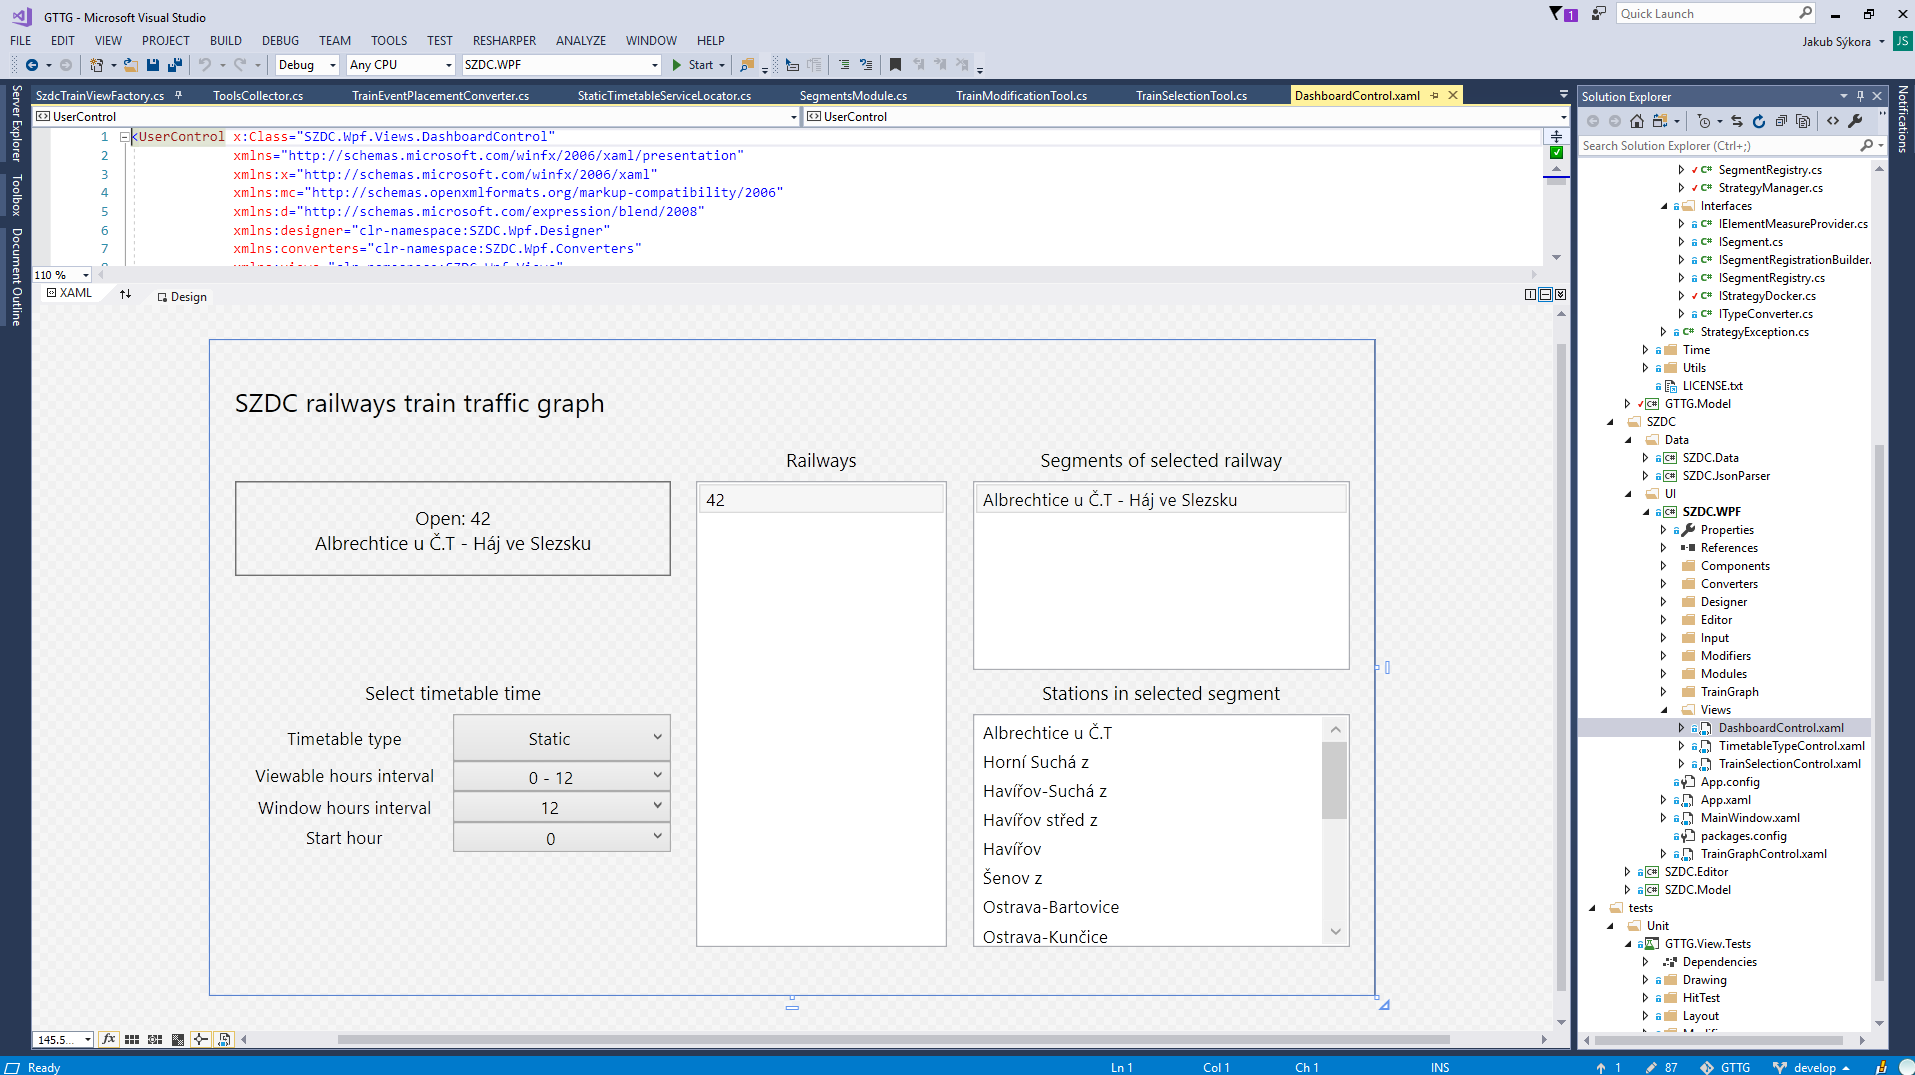
\includegraphics[width=\textwidth]{../img/kap6_designer_wpf}
	\caption{Designer pro WPF ve Visual Studio 2017}
	\label{fig:kap6:gui_wpf_designer}
\end{figure}

\newpage
\section{Data aplikace SZDC a~její model}
Než jsme mohli začít vytvářet model a~vykreslovat obsah nákresného jízdního řádu, museli jsme zjistit, podle jakých pravidel se nákresný jízdní řád Správy železniční a~dopravní cesty vytváří a~s~jakými daty pracuje. Na základě získaných dat jsme poté vytvořili jejich zdroj, ke kterému se může aplikace připojit a~používat je. Pravidla popisující tvorbu grafikonu vlakové dopravy se nachází v~článku 13 dokumentu Směrnice SŽDC č. 69, dostupném jako \texttt{podklady-njr.pdf} v~příloze práce v~\texttt{/szdc/documents/}. Naším cílem bylo co nejvíce těchto pravidel vizualizovat. Potřebujeme ale data, na která je pravidla možné aplikovat. Data, která jsou zobrazována v~nákresných jízdních řádech, jsou dostupná online jako PDF dokumenty představující knižní a~sešitové jízdní řády \cite{GVD_sjr}. Pro nahlédnutí se nachází v~příloze práce v~\texttt{/szdc/sjr/}. Data ve formátech pro strojové zpracování jako je třeba JSON bohužel nejsou veřejně dostupná. Proto jsme se rozhodli najít cestu, jak získat data z~PDF souborů. Na základě zpracovaných dat jsme pak určili konkrétní podporovaná pravidla.

Celá jízda jednoho vlaku, který je označen unikátním číslem, je rozdělena do několika sešitových jízdních řádů určených pro konkrétní tratě. Každý obsahuje pouze nějakou část jeho celého plánu jízdy, jako na obrázku \ref{fig:kap6:sjr_plan_jizdy}. Sloupce 5 a~7 odpovídají příjezdu a~odjezdu do dopravního bodu. Dokument \texttt{tabulka-sjr.pdf} v~příloze práce v~\texttt{/szdc/documents/} tuto tabulku plánu jízdy vlaku v~sešitovém jízdním řádu detailně popisuje.

\begin{figure}[!hbt]
	\centering
	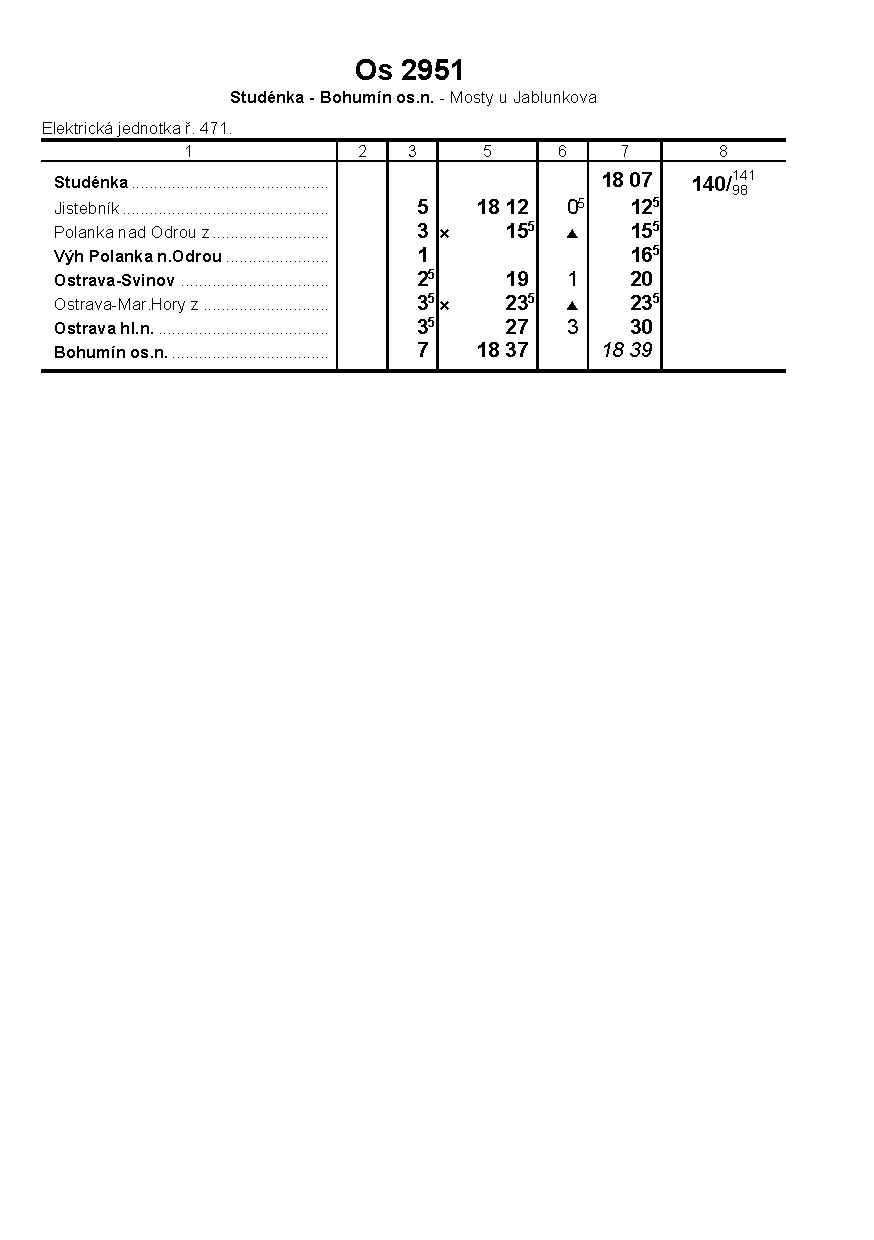
\includegraphics[width=\textwidth]{../img/kap6_sjr_plan_jizdy}
	\caption{Část plánu jízdy vlaku 2951 v~sešitovém jízdním řádu}
	\label{fig:kap6:sjr_plan_jizdy}
\end{figure}

Rozhodli jsme se, že PDF soubory sešitových jízdních řádů naparsujeme, převedeme do vhodného formátu a~získáme z~nich části plánu jízd vlaku, které pak sloučíme do jednoho celého plánu. Až budeme vytvářet nákresný jízdní řád, vlaky v~něm získáme průnikem stanic se stanicemi v~takto sloučených plánech.

Tabulková data ze sešitových jízdních řádů jsme se pokoušeli získat pomocí různých PDF nástrojů, ale ukázalo se, že tabulky jsou pro zpracování nějakým frameworkem pro práci s~PDF soubory příliš komplexní. Vyzkoušeli jsme, jak tyto tabulky vypadají po převodu do tabulkového XLSX formátu. Data v~tomto formátu se ukázala být již lépe zpracovatelná. Jelikož jsme měli zkušenost s~parsováním XLSX souborů pomocí knihovny Apache POI~\cite{Apache_POI} v~Javě, rozhodli jsme se soubory zpracovat touto knihovnou. Výsledkem zpracování je vygenerovaný JSON výstup, uvedený na následujícím fragmentu kódu. Čas se uvádí v~půlminutách ve vlastnosti \texttt{"isAfter30Seconds"} odpovídající číslu pět v~horním indexu za minutovým údajem ve sloupcích příjezdu (5) a~odjezdu (7), které se seznamem stanic v~prvním sloupci zpracováváme.

\begin{csharpcode}
{ "trains": {
  "2951": {
	"trainType": "Os",
    "schedule": [
      {
        "departureTime": {
          "hours": 18,
          "minutes": 7,
          "isAfter30Seconds": false
        },
        "arrivalTime": null,
        "stationName": "Studénka"
      },
      { (+) },
      .
      .
      .
	  { (+) },
      ]
   },
   "1345": { (+) }
}
}
\end{csharpcode}

Jiná data v~dalších sloupcích sešitových jízdních řádů nezpracováváme, z~důvodu jejich nespolehlivého převedení do XLSX souboru. Příklad převedeného sešitového jízdního řádu do souboru XLSX a~vytvořené Java aplikace pro jeho parsování se nachází v~příloze práce v~\texttt{/szdc/parser/xlsx}. Pomocí tohoto postupu jsme z~celkového počtu přibližně 20000 plánů nedokázali získat řádově desítky plánů jízd. Všechny takto úspěšně převedené plány jízd se nachází v~příloze práce v~\texttt{/szdc/njr/json}. Ve formátu JSON se vytváří i~popis traťových úseků v~rámci nákresného jízdního řádu, jako v~souboru \texttt{/szdc/njr/json/railways/301.json}.

Pro parsování JSON dat do různých aplikací je vývojářům dostupná utilita \texttt{SZDC.JsonParser}, která převádí tato data formátu JSON do objektů C\#. Parseru se předává objekt knihovny Newtonsoft~\cite{Newtonsoft}, představující načtený JSON soubor. Data jsou parserem předána implementaci rozhraní \texttt{IParsedTrainReceiver}, kterou parseru dodá vývojář. Stejným způsobem jsou pak získatelná data popisující stanice.

\subsection*{Pravidla pro sestavení nákresného jízdního řádu}
Nyní si na základě dostupných dat představíme pravidla, která podporujeme, podle článku 13 Směrnice SŽDC č. 69, ilustrovaná obrázky v~\ref{fig:kap6:szdc_koty} a nacházející se v příloze \texttt{/szdc/documents/podklady-njr.pdf}:

\begin{figure}[ht]
    \centering
    \begin{subfigure}[b]{0.24\textwidth}
        
\includegraphics[width=0.7\textwidth]{../img/koty_dalsi_set_y}
        \caption{}
        \label{fig:kap6:szdc_koty_y}
    \end{subfigure}
    \begin{subfigure}[b]{0.24\textwidth}
        
\includegraphics[width=0.7\textwidth]{../img/koty_dalsi_set_z}
        \label{fig:kap6:szdc_koty_z}
        \caption{}
    \end{subfigure}
	\begin{subfigure}[b]{0.24\textwidth}
        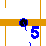
\includegraphics[width=0.7\textwidth]{../img/koty_dalsi_set_a}
        \label{fig:kap6:szdc_koty_a}        
        \caption{}
    \end{subfigure}
	\begin{subfigure}[b]{0.24\textwidth}
        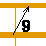
\includegraphics[width=0.7\textwidth]{../img/koty_dalsi_set_b}
        \label{fig:kap6:szdc_koty_b}
        \caption{}
    \end{subfigure}
    
    \caption{Ilustrace pravidel tvorby nákresného jízdního řádu.}
    \label{fig:kap6:szdc_koty}    
\end{figure}

\begin{quote}
\textit{
\begin{itemize}
	\item[13.2.2] Trasy vlaků osobní dopravy (zkratky Os, Sp, R, Ex) se tisknou černě, trasy vlaků nákladní dopravy a~služebních vlaků (zkratky Nex, Mn, Sl, Vl, Pn) modře.
	\item[13.2.2] Kóty, čísla vlaků a~příp. značky před kótami se tisknou stejnou barvou jako trasa vlaků.
	\item[13.3.2] Trasy nákladních vlaků se ve výchozích a~konečných stanicích označí zakreslením plného kolečka na vodorovné čáře stanice (c).
	\item[13.2.10] Projíždí-li vlak v~odbočné stanici nebo na odbočce na jinou trať nebo projíždí-li stanici ohraničující zobrazený úsek, prodlouží se trasa krátkou šipkou k~umožnění zapsání průjezdové kóty (d). Obdobně se vyznačí průjezd vlaku vstupujícího v~odbočné stanici nebo ve stanici ohraničující zobrazený úsek.
	\item[13.2.12] U~příjezdových kót v~dopravnách a~stanovištích se používají\linebreak značky pro vyznačení:
		\begin{enumerate}
			\item Pobytu kratšího než půl minuty. Kóta se nahradí trojůhelníkem jako v~(a)
		\end{enumerate}
\end{itemize}}
\end{quote}

Pokud má časový údaj o~půl minuty více, kóta se podtrhává (b). Síla čar trasy vlaku je určena na obrázku \ref{fig:kap6:tloustka_car_trasy_vlaku} podle zkratek zmíněných v~pravidle 13.2.2.

\begin{figure}[!hbt]
	\centering
	
\includegraphics[width=\textwidth]{../img/kap6_tloustka_car_trasy_vlaku}
	\caption{Tloušťky čar představující trasy vlaku}
	\label{fig:kap6:tloustka_car_trasy_vlaku}
\end{figure}

\subsection*{Práce s~daty a~SZDC.Data}
Jako zdroj dat slouží aplikaci projekt \texttt{SZDC.Data}, který importuje data ve zmíněném JSON formátu a~nahrává je do PostgreSQL~\cite{PostgreSQL} databáze pomocí EntityFrameworkCore~\cite{EntityFrameworkCore}. Projekt implementuje rozhraní \texttt{IStaticDataProvider} v~třídě \texttt{DbDataProvider}, pomocí kterého aplikace získává z~\texttt{SZDC.Data} data. V~rámci představení možností práce s~knihovnou jsme ke každé stanici při parsování dat, které probíhá pomocí konzolové aplikace v~tomto projektu, navíc vygenerovali její koleje.

Pokud chce vývojář dodat aplikaci vlastní databázi jako zdroj dat, v~příloze práce v~\texttt{/szdc/db} se nachází návod, jak propojit aplikaci s~databází, inicializovat ji používaným schématem modelu a~importovat do ní data ve formátu JSON. 

\newpage
\subsection*{Model a~view model aplikace}
Pravidla, podle kterých chceme obsah zobrazovat, jsme zahrnuli do modelu vytvořeném v~projektu \texttt{SZDC.Model}, který dále rozšiřuje základní model \linebreak z~knihovny GTTG. Implementovaný view model v~tomto projektu pak s~vlastnostmi modelu představující pravidla pracuje. Například tloušťka a~vlastnosti čar se view modelům přiřazují v~implementaci factory metod. Pokud se musí aplikovat pravidla 13.3.2 a~13.2.10 související s~přidáváním prvků vizualizace trasy vlaku, používáme \textit{decorator} pattern řetězením několika implementací rozhraní \texttt{ITrainPath}, každé dodávající vizualizaci nějakého pravidla.

Pravidla spojená s~vizualizací kót jsou implementována různými zobrazitelnými prvky. V~přetížené metodě \texttt{UpdateTrainViewContent()} na view modelu \linebreak vlaku \texttt{SzdcTrainView} každé jeho události \texttt{SzdcTrainEvent} nastavíme \textit{flagy} \linebreak výčtového typu \texttt{TrainEventFlags} -- například \texttt{LessThanHalfMinute} pro nahrazení číselné kóty trojúhelníkem podle 13.2.12. Dále se pak v~této metodě podle kombinace flag každé události přidělí zobrazitelný prvek reprezentující kótu -- například \texttt{TimeComponent} nebo \texttt{TriangleComponent}. Tyto prvky se pak v~metodě \texttt{Arrange()} spolu s~čísly vlaků rozmístí podle strategií základní implementace zmíněných v~\ref{kap4:strategy}.

\section{Uživatelská dokumentace}
\label{kap6:szdc:user_doc}
V~této podkapitole si ukážeme možnosti práce s~aplikací SZDC na dvou módech nabízených aplikací. Při spuštění aplikace se uživateli zobrazí okno na obrázku \ref{fig:kap6:szdc_menu}, pomocí kterého uživatel otevírá nová okna s~nákresným jízdním řádem.

\begin{figure}[!hbt]
	\centering
	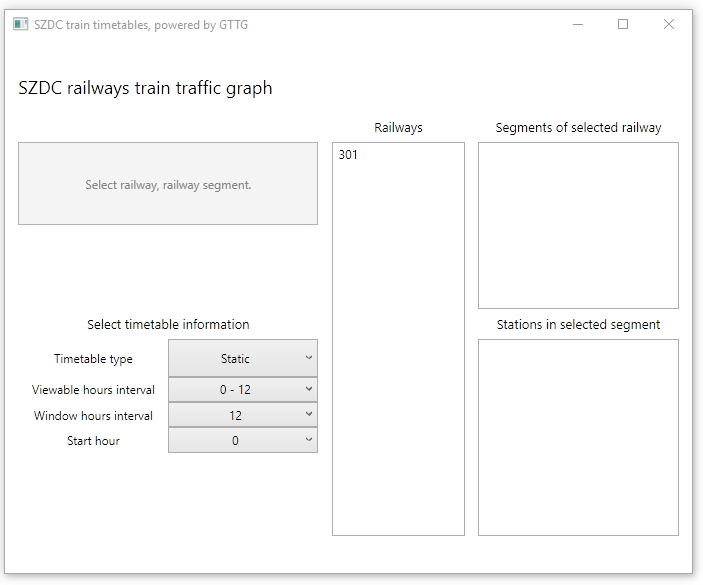
\includegraphics[width=.8\textwidth]{../img/kap6_szdc_menu}
	\caption{Okno pro otevření nákresného jízdního řádu v aplikaci SZDC}
	\label{fig:kap6:szdc_menu}
\end{figure}

\newpage
Ve sloupci \texttt{'Railways'} se nachází seznam očíslovaných tratí. Když na číslo v~seznamu klikneme, ve sloupci \texttt{'Segments of selected railway'} se uživateli zobrazí úseky tratě (na obrázku \ref{fig:kap6:szdc_menu_select}), podle obsahu nákresného jízdního řádu zvolené trati. Například pro trať číslo 301 se uživateli nabízí zvolit pět úseků, nacházejících se v~nákresném jízdním řádu v~příloze práce v~\texttt{/szdc/njr/pdf/L301\_d.pdf}. Kliknutím na vybraný úsek se ve sloupci \texttt{'Stations in selected segment'} zobrazí jeho seznam dopravních bodů.

\begin{figure}[!hbt]
	\centering
	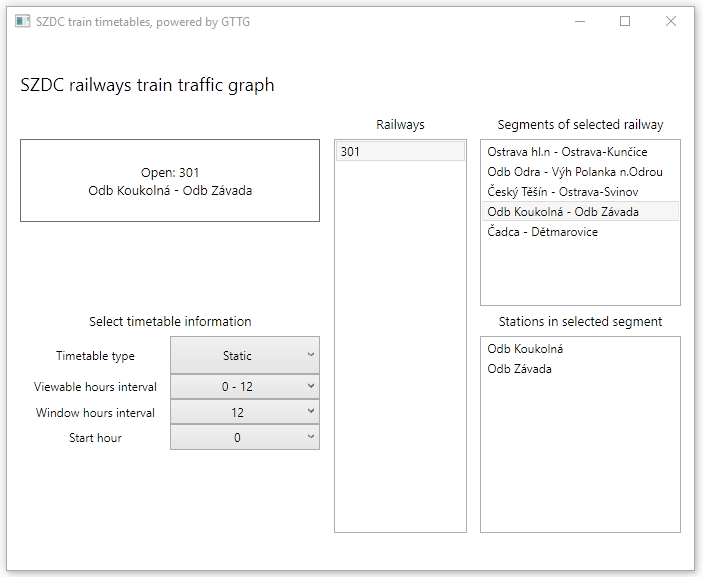
\includegraphics[width=\textwidth]{../img/kap6_szdc_menu_select}
	\caption{Otevření nákresného jízdního řádu v~aplikaci SZDC}
	\label{fig:kap6:szdc_menu_select}
\end{figure}

Tlačítko v~levé horní části okna, určené k~otevření okna nákresného jízdního řádu, se tímto výběrem nachází ve stavu, kdy text tlačítka obsahuje číslo vybrané trati a~jejího úseku. Kliknutím na tlačítko se otevře nové okno s~vybraným nákresným jízdním řádem. Pod tlačítkem se nachází oblast \texttt{'Select timetable information'}, v které konfigurujeme otevíraný nákresný jízdní řád. V~kombinovaném seznamu \texttt{'Timetable type'} se vybírá jeden z~módů zobrazení nákresného jízdního řádu \texttt{'Static'} a~\texttt{'Realtime'}, které si představíme v~dalších částech. Pro \texttt{'Static'} mód je možné vybrat určením času zobrazovaný obsah. Kombinovaný seznam \texttt{'Viewable hours interval'} udává časový rozsah, který je možné prohlížet. \texttt{'Window hours interval'} nastavuje počáteční délku zobrazovaného časového intervalu. \texttt{'Start hour'} udává hodinu, kterou bude začínat časový interval zobrazení v okně při otevření.

\newpage
\subsection*{Statický mód zobrazení nákresného jízdního řádu}
Nyní si popíšeme okno, které se otevře při nastavení hodnoty kombinovaného seznamu \texttt{'Timetable type'} na \texttt{'Static'}. Okno nákresného jízdního řádu ve statickém módu se nachází na obrázku  \ref{fig:kap6:static_mode} a umožňuje pouze prohlížení nákresného jízdního řádu. Skrolováním myši je možné pohled oddalovat a~přibližovat. Držením levého tlačítka při posunu myši je možné měnit zobrazovaný obsah. Časový interval, který je možné zobrazit, je uveden v~\texttt{'Viewable interval'}. Zobrazený časový interval je možné měnit pomocí \texttt{'Select time'}. Pohybem myši po obsahu nákresného jízdního řádu se v levém horním rohu ukazuje čas odpovídající pozici kurzoru.

\begin{figure}[!hbt]
	\centering
	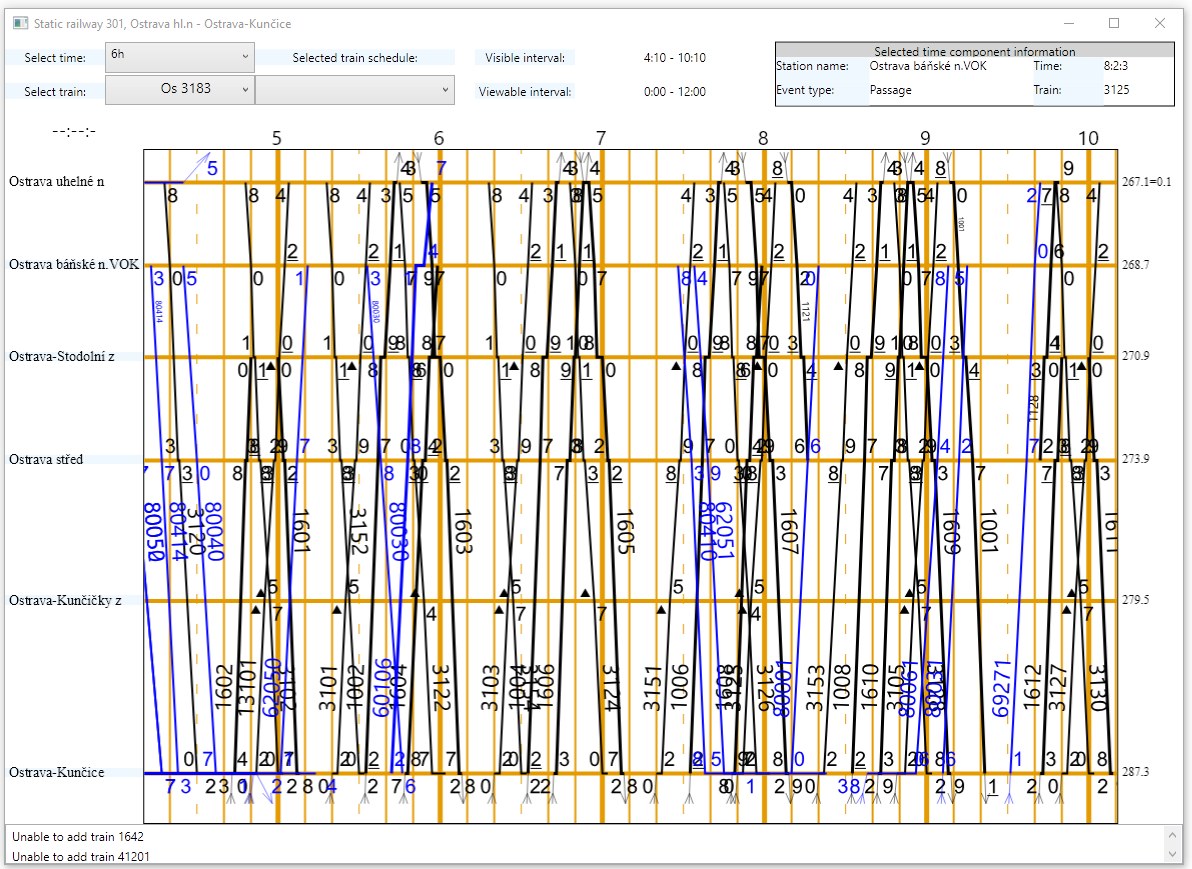
\includegraphics[width=\textwidth]{../img/kap6_static_timetable}
	\caption{Nákresný jízdní řád ve statickém módu}
	\label{fig:kap6:static_mode}
\end{figure}

\begin{figure}[!hbt]
	\centering
	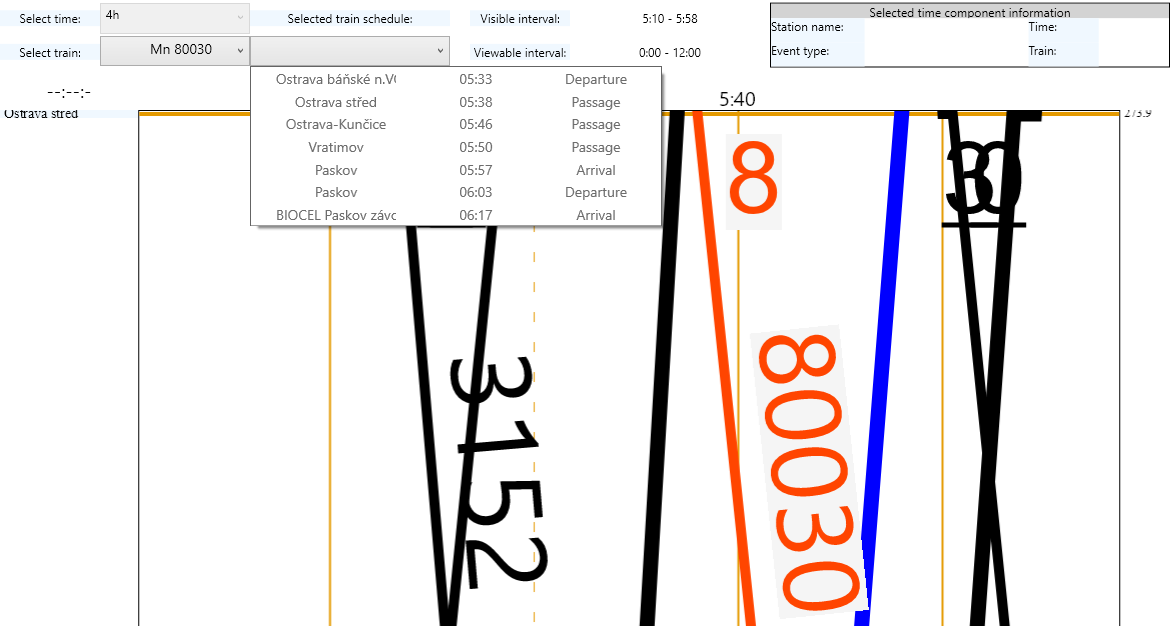
\includegraphics[width=\textwidth]{../img/kap6_static_schedule_train_selection}
	\caption{Zobrazený průběh jízdy vybraného vlaku}
	\label{fig:kap6:static_schedule_train_selection}
\end{figure}

Kliknutím na kombinovaný seznam označený \texttt{'Select train'} je možné vybrat vlak, který je pak v~obsahu nákresného jízdního řádu oranžově zvýrazněn a~přenesen do popředí, jako na obrázku \ref{fig:kap6:static_schedule_train_selection}. Navíc jsou jeho kóty a číslo vlaku pro větší přehlednost bíle podbarvené. Výběr vlaku je možné provést i~kliknutím pravým tlačítkem na obsah nákresného jízdního řádu, kdy se vybere nejbližší vlak k~pozici kurzoru myši. Otevřením seznamu pod \texttt{'Selected train schedule'} se otevře plán jízdy vlaku. Kliknutím levého tlačítka na kótu se zobrazí podrobnější informace v~\texttt{'Selected time component information'} -- typ události (příjezd, odjezd, průjezd), stanice, číslo vlaku a~čas.

Pokud dopravní bod obsahuje více kolejí, je jeho jméno v~levém sloupci modře podbarvené. Kliknutím na toto podbarvení je možné horizontální čáru dopravního bodu rozdělit do více kolejí, jako na obrázku \ref{fig:kap6:szdc_toggle_stations}. Toto rozdělení je pak znovu možné seskupit do jedné čáry kliknutím na podbarvení.

\begin{figure}[!hbt]
	\centering
	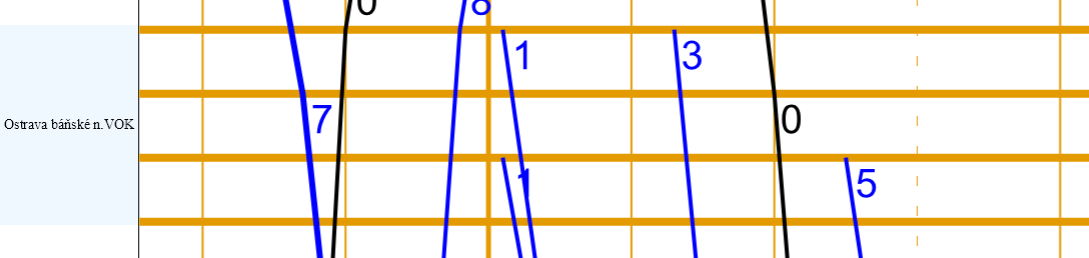
\includegraphics[width=\textwidth]{../img/kap6_szdc_toggle_stations}
	\caption{Rozdělení vodorovné čáry dopravního bodu do jednotlivých kolejí}
	\label{fig:kap6:szdc_toggle_stations}
\end{figure}

\subsection*{Dynamický mód zobrazení nákresného jízdního řádu}
Dynamický mód, jehož okno se nachází na obrázku \ref{fig:kap6:dynamic_schedule}, nabízí stejné nástroje jako statický mód a~navíc umožňuje modifikaci plánovaného průběhu jízd vlaků. Aplikace sama v~krátkých časových intervalech upravuje náhodně průběh jízdy některých vlaků. Při změnách se mění hodnoty časových kót i~jejich zobrazení podle uváděných pravidel. Pokud je otevřeno více oken dynamického módu, které zobrazují stejný vlak, změny se zobrazí ve všech oknech. Zobrazuje se aktuální časový interval délky osmi hodin a průběžně se po hodině posouvá. Při posunu jsou přidávána i~odebírána zobrazovaná data. Zelená svislá čára se obnovuje každou minutu a~značí aktuální čas.

\begin{figure}[!hbt]
	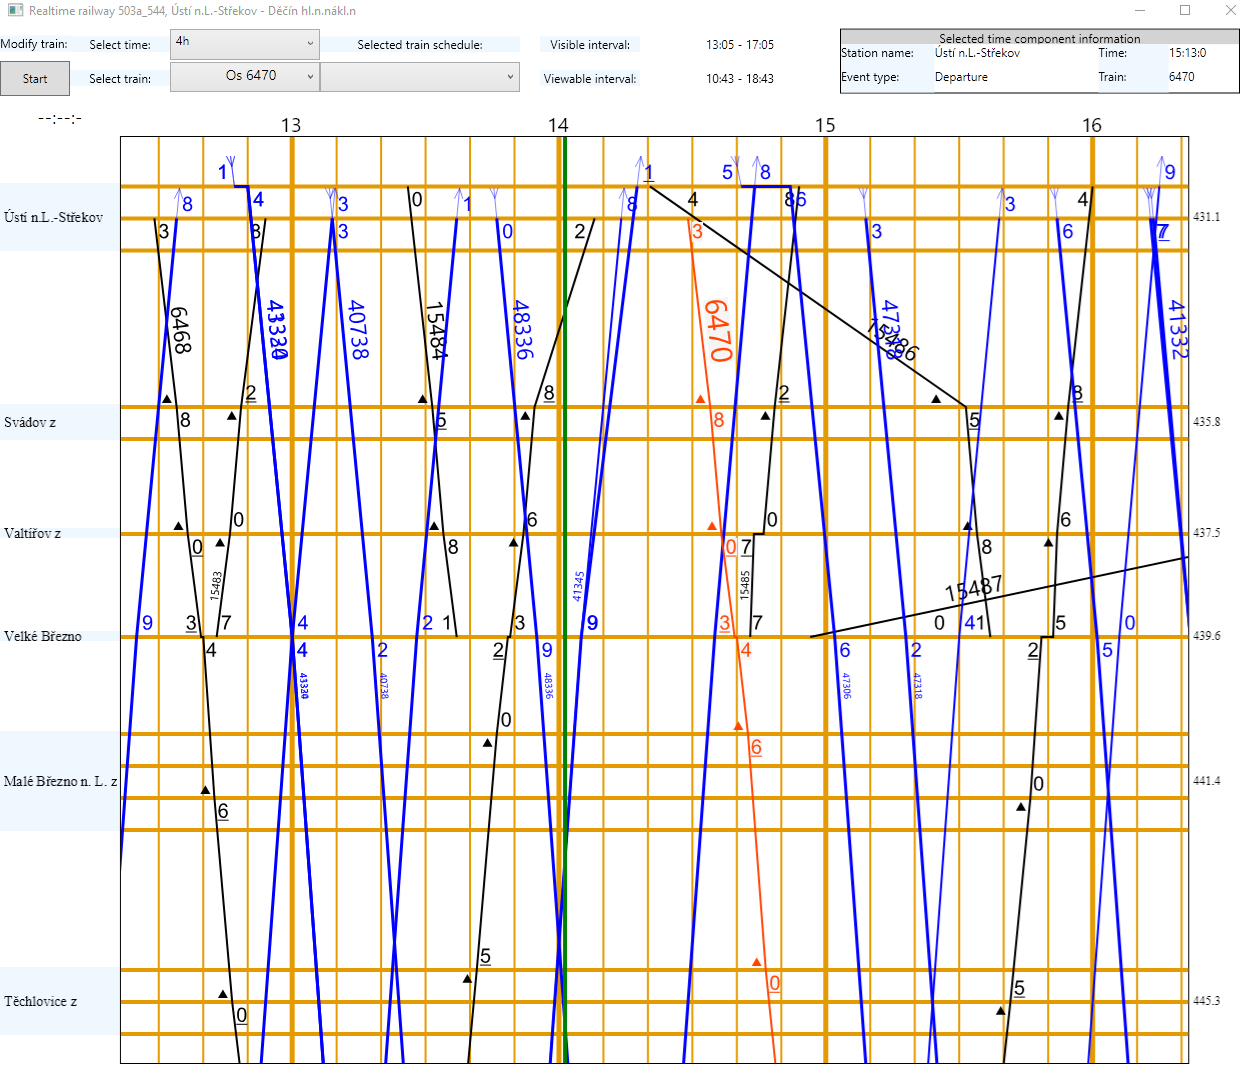
\includegraphics[width=\textwidth]{../img/kap6_dynamic_schedule}
	\caption{Dynamický mód zobrazení v~aplikaci SZDC}
	\label{fig:kap6:dynamic_schedule}
\end{figure}

Po kliknutí na tlačítko pod textem \texttt{'Modify train'} v~horní liště okna může uživatel sám interaktivně měnit plán jízd vlaků. Nejdříve musí uživatel vlak vybrat, aby se nacházel v~\texttt{'Select train'}. Poté uživatel klikne na zmíněné tlačítko. Není možné již provádět pravým tlačítkem výběr jiných vlaků. Naopak klikáním na obsah nákresného jízdního řádu je nyní možné průběh jízdy vlaku upravovat. Na pozici kurzoru myši je přesunuta ta událost, která se k~pozici nachází nejblíže. Úpravy je však možné pouze aplikovat na plánovaný provoz, který se nachází napravo od zelené svislé čáry značící aktuální čas. Modifikace se projeví v ostatních oknech a zároveň i v ostatních uživatelských prvcích okna, jako například v seznamu \texttt{'Selected train schedule'}.

